\documentclass{article}
\usepackage{ae,aecompl}
\usepackage{todonotes}
\usepackage{chngcntr}
\usepackage{tikz-cd}
\usepackage{graphicx}
\graphicspath{ {./images/}}
\usepackage[all,cmtip]{xy}
\usepackage{amsmath, amscd}
\usepackage{amsthm}
\usepackage{amssymb}
\usepackage{amsfonts}
\usepackage{bm}
\usepackage{qsymbols}
\usepackage{latexsym}
\usepackage{mathrsfs}
\usepackage{mathtools}
\usepackage{cite}
\usepackage{color}
\usepackage{url}
\usepackage{enumerate}
\usepackage{verbatim}
\usepackage[draft=false, colorlinks=true]{hyperref}
\usepackage{pdfpages}
\usepackage[margin=1.2in]{geometry}
\usepackage{IEEEtrantools}

\usepackage{fancyhdr}


\usepackage[nameinlink]{cleveref}


\DeclareMathOperator*{\ac}{accept}
\DeclareMathOperator*{\amax}{argmax}
\DeclareMathOperator*{\amin}{argmin}
\DeclareMathOperator*{\Aut}{Aut}
\newcommand {\al}{{\alpha}}
\newcommand {\abs}[1]{{\left\lvert#1\right\rvert}}
\newcommand {\A}{{\mathcal{A}}}
\newcommand {\AM}{{\mathrm{AM}}}
\newcommand {\AMp}{{\AM_{p}^{X}\!(\Ri_\w)}}
\newcommand {\B}{{\mathcal{B}}}
\DeclareMathOperator*{\Be}{Bern}
\newcommand {\Br}{{\dot{B}}}
\newcommand {\Ba}{{\mathfrak{B}}}
\newcommand {\C}{{\mathbb C}}
\newcommand {\ce}{\mathrm{c}}
\newcommand {\Ce}{\mathrm{C}}
\newcommand {\Cc}{\mathrm{C_{c}}}
\newcommand {\Ccinf}{\mathrm{C_{c}^{\infty}}}
\DeclareMathOperator{\cov}{Cov}
\DeclareMathOperator{\DEV}{DEV}
\newcommand {\Di}{{\mathbb D}}
\newcommand {\dom}{\mathrm{dom}}
\newcommand{\dist}{\stackrel{\mathrm{dist}}{=}}
\newcommand {\ud}{\mathrm{d}}
\newcommand {\ue}{\mathrm{e}}
\newcommand {\eps}{\varepsilon}
\newcommand {\veps}{\varepsilon}
\newcommand {\vrho}{{\varrho}}
\newcommand {\E}{{\mathbb{E}}}
\newcommand {\Ec}{{\mathcal{E}}}
\newcommand {\Ell}{L}
\newcommand {\Ellp}{{L_{p}[0,1]}}
\newcommand {\Ellpprime}{{L_{p'}([0,1])}}
\newcommand {\Ellq}{{L_{q}([0,1])}}
\newcommand {\Ellqprime}{{L_{q'}([0,1])}}
\newcommand {\Ellr}{L^{r}}
\newcommand {\Ellone}{{L_{1}([0,1])}}
\newcommand{\Elltwo}{{L_{2}([0,1])}}
\newcommand{\Ellinfty}{L^{\infty}}
\newcommand{\Ellinftyc}{L_{\mathrm{c}}^{\infty}}
\newcommand{\exb}[1]{\exp\left\{#1\right\}}
\DeclareMathOperator*{\Ext}{Ext}
\newcommand{\F}{{\mathcal{F}}}
\newcommand{\Fe}{{\mathbb{F}}}
\newcommand{\G}{{\mathcal{G}}}
\newcommand{\HF}{\mathcal{H}_{\text{FIO}}^{1}(\Rd)}
\newcommand{\Hr}{H}
\newcommand{\HT}{\mathcal{H}}
\newcommand{\ui}{\mathrm{i}}
\newcommand{\I}{{I}}
\newcommand{\J}{{\mathcal{J}}}
\newcommand{\id}{{\mathrm{id}}}
\newcommand{\iid}{\stackrel{\mathclap{\normalfont\mbox{iid}}}{\sim}}
\newcommand{\im}{{\text{im }}}
\newcommand{\ind}{{\perp\!\!\!\perp}}
\DeclareMathOperator*{\Int}{int}
\newcommand{\intx}{{\overline{\int_{X}}}}
\newcommand{\inte}{{\overline{\int_{\E}}}}
\newcommand{\la}{\lambda}
\newcommand{\rb}{\rangle}
\newcommand{\lb}{{\langle}}
\newcommand{\La}{\Lambda}
\newcommand{\calL}{{\mathcal{L}}}
\newcommand{\lp}{{\mathcal{L}}^{p}}
\newcommand{\lpo}{{\overline{\mathcal{L}}^{p}\!}}
\newcommand{\Lpo}{{\overline{\Ell}^{p}\!}}
\newcommand{\M}{{\mathbf{M}}}
\newcommand{\Ma}{{\mathcal{M}}}
\newcommand{\N}{{{\mathbb N}}}
\newcommand{\Na}{{{\mathcal{N}}}}
\newcommand{\norm}[1]{\left\|#1\right\|}
\newcommand{\normm}[1]{{\left\vert\kern-0.25ex\left\vert\kern-0.25ex\left\vert #1 
    \right\vert\kern-0.25ex\right\vert\kern-0.25ex\right\vert}}
\newcommand{\Om}{{{\Omega}}}
\newcommand{\one}{{{\bf 1}}}
\newcommand{\pic}{\text{Pic }}
\newcommand{\ph}{{\varphi}}
\newcommand{\Pa}{{\mathbb{P}}}
\newcommand{\Po}{{\mathcal{P}}}
\newcommand{\Q}{{\mathbb{Q}}}
\newcommand{\R}{{\mathbb R}}
\newcommand{\Rd}{{\mathbb{R}^{d}}}
\DeclareMathOperator{\rej}{reject }
\newcommand{\Rn}{{\mathbb{R}^{n}}}
\newcommand{\cR}{{\mathcal{R}}}
\newcommand{\Rad}{{\mathrm{Rad}}}
\newcommand{\ran}{{\mathrm{ran}}}
\newcommand{\Ri}{{\mathrm{R}}}
\newcommand{\supp}{{\mathrm{supp}}}
\newcommand{\Se}{\mathrm{S}}
\newcommand{\Sp}{S^{*}(\Rn)}
\newcommand{\St}{{\mathrm{St}}}
\newcommand{\Sw}{\mathcal{S}}
\newcommand{\T}{{\mathcal{T}}}
\newcommand{\ta}{{\theta}}
\newcommand{\Ta}{{\Theta}}
\newcommand{\topp}{\stackrel{p}{\to}}
\newcommand{\todd}{\stackrel{d}{\to}}
\newcommand{\toL}[1]{\stackrel{L^{#1}}{\to}} 
\newcommand{\toas}{\stackrel{a.s.}{\to}}
\DeclareMathOperator{\V}{Var}
\newcommand {\w}{{\omega}}
\newcommand {\W}{{\mathrm{W}}}
\newcommand {\Wnp}{\text{$\mathrm{W}$\textsuperscript{$n,\!p$}}}
\newcommand {\Wnpeq}{\text{$\mathrm{W}$\textsuperscript{$n\!,\!p$}}}
\newcommand {\Wonep}{\text{$\mathrm{W}$\textsuperscript{$1,\!p$}}}
\newcommand {\Wonepeq}{\text{$\mathrm{W}$\textsuperscript{$1\!,\!p$}}}
\newcommand {\X}{{\mathcal{X}}}
\newcommand {\Z}{{{\mathbb Z}}}
\newcommand {\Za}{{\mathcal{Z}}}
\newcommand {\Zd}{{\Z[\sqrt{d}]}}
\newcommand {\vanish}[1]{\relax}

\newcommand {\wh}{\widehat}
\newcommand {\wt}{\widetilde}
\newcommand {\red}{\color{red}}

% Distributions
\newcommand{\normal}{\mathsf{N}}
\newcommand{\poi}{\mathsf{Poisson}}
\newcommand{\bern}{\mathsf{Bernoulli}}
\newcommand{\bin}{\mathsf{Binomal}}
\newcommand{\multi}{\mathsf{Multinomial}}
\newcommand{\Exp}{\mathsf{Exp}}



% put your command and environment definitions here




% some theorem environments
% remove "[theorem]" if you do not want them to use the same number sequence


  \newtheorem{thrm}{Theorem}
  \newtheorem{lemma}{Lemma}
  \newtheorem{prop}{Proposition}
  \newtheorem{cor}{Corollary}

  \newtheorem{conj}{Conjecture}
  \renewcommand{\theconj}{\Alph{conj}}  % numbered A, B, C etc

  \theoremstyle{definition}
  \newtheorem{defn}{Definition}
  \newtheorem{ex}{Example}
  \newtheorem{exs}{Examples}
  \newtheorem{question}{Question}
  \newtheorem{remark}{Remark}
  \newtheorem{notn}{Notation}
  \newtheorem{exer}{Exercise}




\title{STATS305B -- Lecture 10}
\author{Jonathon Taylor\\ Scribed by Michael Howes}
\date{02/07/22}

\pagestyle{fancy}
\fancyhf{}
\rhead{STATS305B -- Lecture 10}
\lhead{02/07/22}
\rfoot{Page \thepage}

\begin{document}
\maketitle
\tableofcontents
\section{Regularized glms}
\subsection{Fitting a ridge glm}
The objective for fitting a glm can be written as
\[\wh{\beta}=\amin_\beta \Lambda(X\beta)-\beta^T(X^TY) = \amin_\beta - \log L(\beta|Y). \]
The penalized objective is 
\[\Lambda(X\beta)-\beta^T(X^TY)+\Po(\beta), \]
and the regularized estimator is
\[\wh{\beta}_\Po = \amin_\beta \Lambda(X\beta)-\beta^T(X^TY)+\Po(\beta). \]
One class of penalties are the \emph{ridge penalties}
\begin{align*}
    \Po(\beta)&=\frac{\la}{2}\norm{\beta}_2^2,\\
    \Po(\beta)&= \frac{1}{2}\sum_{j=1}^p \la_j \beta_j^2,\\
    \Po(\beta)&= \frac{1}{2}\beta^TQ\beta,
\end{align*}
where $\la,\la_j > 0$ and $Q$ is symmetric and positive definite. The objective is the function
\[\beta \mapsto \Lambda(X\beta)-\beta^T(X^TY)+\frac{1}{2}\beta^TQ\beta. \]
To minimize this objective function we can do Newton--Raphson. Some calculus gives that the iterates are given by 
\[\wh{\beta}^{(t+1)}=\wh{\beta}^{(t+1)}-(X^TW^{(t-1)}X+Q)^{-1}(X^TW^{(t-1)}g'(\wh{u}^{(t-1)})(\wh{\mu}^{t-1}-Y)+Q\wh{\beta}^{(t-1)}). \]
There are other iterative fitting methods.
\subsection{Why regularize}
Suppose we are fit a model regularized with standard ridge regression so that $\Po(\beta)=\frac{\la}{2}\norm{\beta}_2^2$. Consider the simple Gaussian case with unit variance. This means that $Y \sim \normal(X\beta,  I_n)$. The bias of the ridge estimator is 
\[\text{Bias}(\wh{\beta}_\la) = \norm{\E[\wh{\beta}_\la]-\beta}_2^2 = \la^2 \sum_{j=1}^p \frac{\al_j^2}{(d_j^2+\la)^2}. \]
And the variance satisfies
\[\text{tr}(\V(\wh{\beta}_\la)) = \sum_{j=1}^p \frac{d_j^2}{(d_j^2+\la)^2} \le \sum_{j=1}^p \frac{1}{d_j^2}. \]
The values $d_j$ are the singular values of $X$ and $\al_j = \beta^Tv_j$ where $v_j$ is the $j^{th}$ singular vector of $X = UDV^T$. Thus, when compared to the OLS estimator, the ridge estimator has higher bias but lower variance. Combining these gives
\[\E[\norm{\wh{\beta}_\la-\beta}_2^2] = \la^2 \sum_{j=1}^p \frac{\al_j^2}{(\al_j^2+\la)^2}+\sum_{j=1}^p \frac{d_j^2}{(d_j^2+\la)^2}.\]
By differentiating the above one can find $\la^*$ which is the value of $\la$ that minimizes the expected square error. It turns out that $\la^* > 0$ and the expected square error is always decreasing at $\la = 0$. This means that doing a small amount of ridge regularization will decrease the expected square error. Unfortunately finding the optimal $\la$ depends on $\al_j$, and we do not know $\al_j$. Thus, in practice, a value of $\la$ is chosen based on cross validation. 
\section{LASSO regularization}
\subsection{The LASSO in one dimension}
Consider the penalty
\[\Po(\beta)= \la \norm{\beta}_1 = \la \sum_{j=1}^p \abs{\beta_j}. \]
Let's see what this penalty does in a one dimensional problem. Consider
\[\wh{\beta}= \amin_\beta \frac{1}{2}(Z-\beta)^2+\la\abs{\beta}. \]
If $\la = 3$, $Z=2$, then the objective becomes
\begin{align*}
    \frac{1}{2}(2-\beta)^2+3\abs{\beta} &= \frac{1}{2}\beta^2 - 2\beta +2+3\abs{\beta}\\
    &=\begin{cases}
        \frac{1}{2}\beta^2 +\beta+2 & \text{if } \beta \ge 0,\\
        \frac{1}{2}\beta^2 - 5\beta + 2 & \text{if } \beta < 0.
    \end{cases}
\end{align*}
The objective looks like this
\begin{center}
    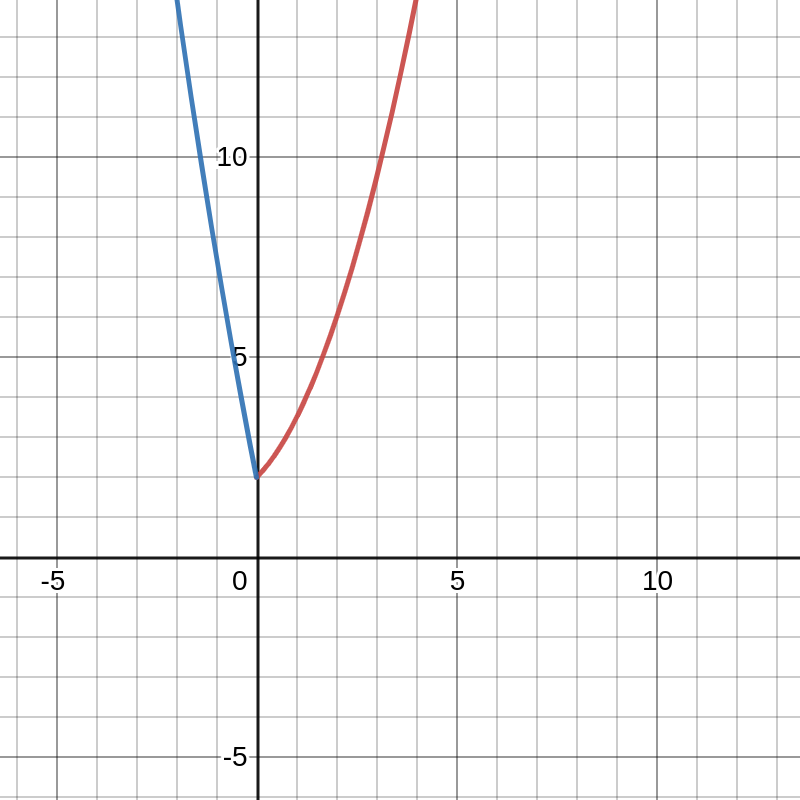
\includegraphics[width = 0.3\textwidth]{lec10_01.png}
\end{center}
Thus, the minimum occurs at $\la = 0$. If $\la =3$ and $Z=4$, then the objective is 
\begin{align*}
    \frac{1}{2}(4-\beta)^2+3\abs{\beta} &= \frac{1}{2}\beta^2 - 4\beta + 8 + 3\abs{\beta} \\
    &=\begin{cases}
        \frac{1}{2}\beta^2 - \beta + 8 & \text{if } \beta \ge 0,\\
        \frac{1}{2}\beta^2 -7\beta + 8 & \text{if } \beta <0.
    \end{cases}
\end{align*}
So the objective looks like this
\begin{center}
    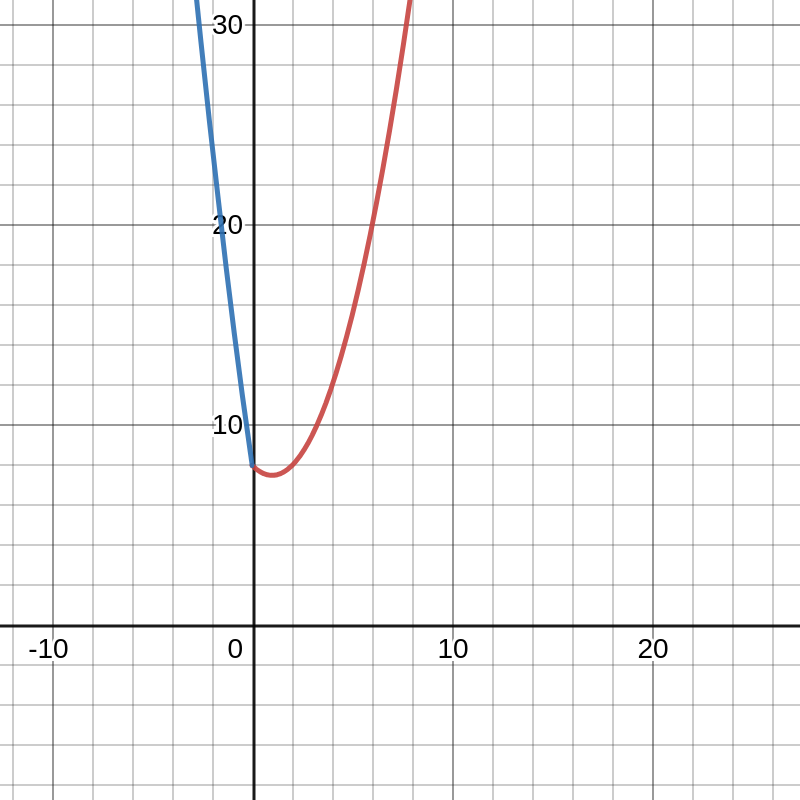
\includegraphics[width = 0.3\textwidth]{lec10_02.png}
\end{center}
The minimum occurs at $\beta = 1$. In general, consider the objective \[g_z(\beta) = \frac{1}{2}(\beta-z)^2 + \la\abs{\beta}. \]
This objective function is differentiable at all points other than $\beta = 0$ and for $\beta \neq 0$, 
\[\frac{d}{d\beta}g_z(\beta) = \beta - z + \la \sign(\beta), \]
where
\[\sign(\beta) =\begin{cases}
    1 & \text{if } \beta > 0,\\
    -1 & \text{if } \beta < 0.
\end{cases} \]
Solving $\frac{d}{d\beta}g_z(\beta) = 0$ implies that $\beta = z+\la\sign(\beta)$. This equation has a solution if and only if $\abs{z} \ge  \la$. When $z \ge \la$, the solution is $\wh{\beta}_\la(z) = z-\la$ and when $z \le -\la$, the  solution is $\wh{\beta}_\la(z)=z+\la$. When the equation $\frac{d}{d\beta} g_z(\beta)=0$ has no solutions, the minimizer must occur at $0$. Therefor, we have 
\begin{align*}
    \wh{\beta}_\la(z) &= \amin_\beta \frac{1}{2}(z-\beta)^2+\la\abs{\beta} \\
    &=\begin{cases}
        z+\la & \text{if } z \le - \la,\\
        0 & \text{if } -\la < z < \la,\\
        z-\la & \text{if } z \ge \la.
    \end{cases}\\
    &=:S_\la(z).
\end{align*}
The function $S_\la(z)$ is called the soft-threshold function. For $\la = 5$, it looks like this
\begin{center}
    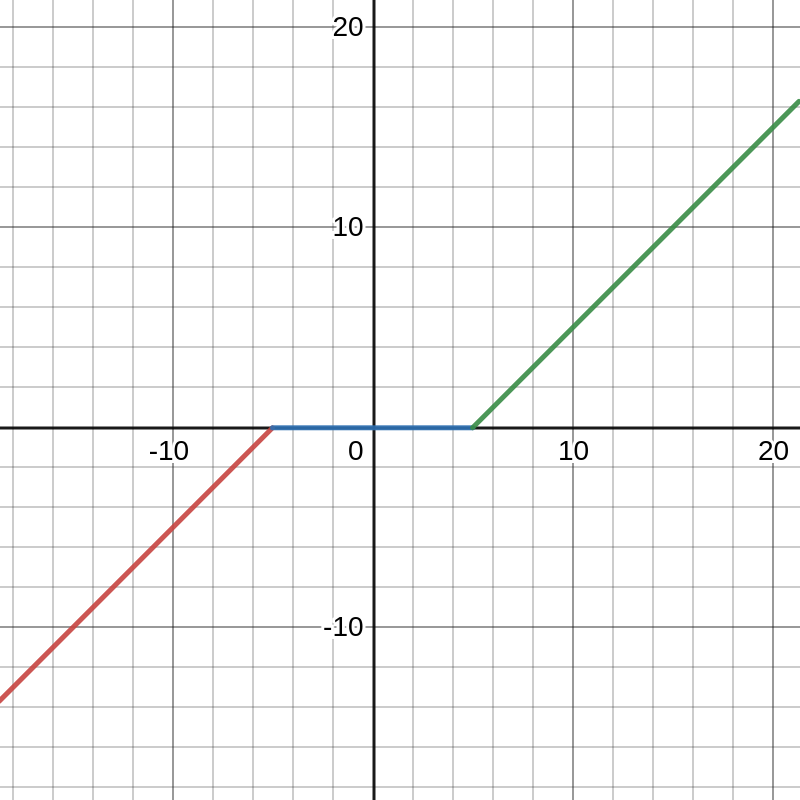
\includegraphics[width = 0.5\textwidth]{lec10_03.png}
\end{center}
One way to write the soft threshold function is  
\[S_\la(z) = \sign(z)\max(\abs{z}-\la,0). \]
Part of this argument generalizes to functions other that $\frac{1}{2}(z-\beta)^2$. Fix a smooth and convex function $f: \R \to \R$ and consider the penalized problem,
\[\wh{\beta}_\la = \amin_\beta f(\beta) + \la \abs{\beta}.  \]
Note that for $\beta \neq 0$,
\[\frac{d}{d\beta} (f(\beta)+\la \abs{\beta}) = f'(\beta)+\la \sign(\beta). \]
We will use this to show that if $\abs{f'(0)} < \la$, then $\wh{\beta}_\la = 0$. Recall that since $f$ is convex and smooth, $f'(\beta)$ is an increasing function. Thus, if $\abs{f'(0)} < \la$, then $f'(0) < \la$ and so $f'(\beta)< \la$ for all $\beta < 0$. Thus, if $\beta < 0$, then 
\[\frac{d}{d\beta} (f(\beta)+\la \abs{\beta}) = f'(\beta)-\la < 0. \]
By a similar argument, if $f'(\beta) > - \la$, then for all $\beta > 0$,
\[\frac{d}{d\beta}( f(\beta)+\la \abs{\beta}) = f'(\beta)+\la > 0. \]
Thus, $\abs{f'(\beta)} < \la$ implies that the first order equation
\[\frac{d}{d\beta}( f(\beta)+\la \abs{\beta} )= 0, \]
has no solutions. And thus we must have $\wh{\beta}_\la = 0$ whenever $\abs{f'(0)}<\la.$ This provides some intuition about what the LASSO penalty sets coefficients equal to zero, and it is also helpful for fitting the LASSO. It provides a quick check for when a coefficient should be zero. 

The graph of $\frac{d}{d\beta} (f(\beta)+\la\abs{\beta})$ when $\abs{f'(0)} < \la$ would like something like this:
\begin{center}
    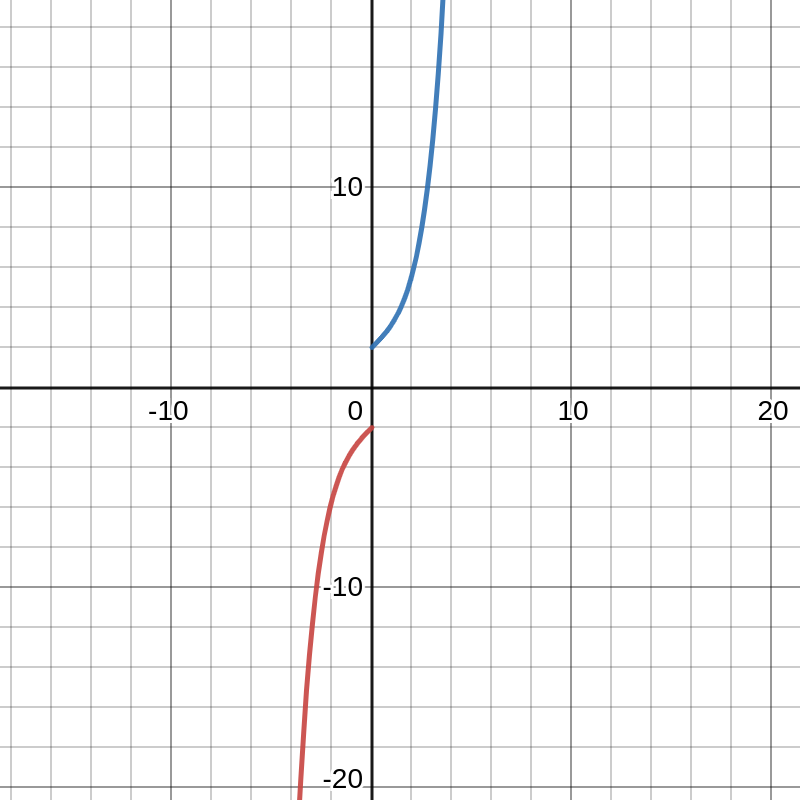
\includegraphics[width = \textwidth/2]{lec10_04.png}
\end{center}
\subsection{Why the LASSO?}
There are other methods that induce sparsity, but the LASSO has the following nice properties.
\begin{itemize}
    \item The minimization problem is convex.
    \item The LASSO minimization problem can be solved for high dimensions.
    \item Since the LASSO minimization problem is convex, the KTT conditions describe the solution. This lets us study LASSO solutions in a way that does not depend on the method used to optimize the LASSO.
\end{itemize}
\subsection{Fitting the LASSO}
We will talk about two iterative methods to fit the LASSO. They are coordinate descent and proximal gradient descent.
\subsubsection{Coordinate descent}
If the penalty $\Po$ was a smooth function, then we could simply use Newton--Raphson to fit the penalized regression. The LASSO penalty is not differentiable at points where one of more $\beta$ coefficient is zero. But, the penalty is \emph{separable}, meaning that 
\[\Po(\beta) = \sum_{j=1}^p \Po_j(\beta_j). \]
For the LASSO we have,
\[\la \norm{\beta}_1 = \sum_{j=1}^p \la \abs{\beta_j}. \]
When the penalty is separable, we can solve penalized regression by iteratively solving a low dimensional problem. More concretely, consider the following procedure
\begin{enumerate}
    \item Start at some $\wh{\beta}^{(0)}$.
    \item At time step $t$, choose an index $j$ and define the univariate objective function,
    \[\beta_j \mapsto f^{(t)}(\beta_j)+\la\abs{\beta_j} = \Lambda(X_{-j}\wh{\beta}_{-j}^{(t)}+X_j\beta_j) -\beta_j(X_j^T)+\la \abs{\beta_j}. \]
    That is, $f^{(t)}(\beta_j)$ is the part of the likelihood that depends on $\beta_j$ when the other coordinates are fixed to equal $\wh{\beta}^{(t)}_{-j}$.
    \item Define $\wh{\beta}^{(t+1)}_j = \amin_{\beta_j}(f^{(t)}(\beta_j)+\la\abs{\beta}_j)$.
    \item Return to step 2 and repeat until convergence.
\end{enumerate}
Some comments
\begin{itemize}
    \item The univariate problem 
    \[ \wh{\beta}^{(t+1)}_j = \amin_{\beta_j}(f^{(t)}(\beta_j)+\la\abs{\beta}_j),\]
    can be solved quickly. One timing saving method is our observation that if $\abs{\frac{d}{d\beta_j}f^{(t)}(\beta_j)} < \la$, then $\wh{\beta}^{(t+1)}_j = 0$.
    \item  If the solution $\wh{\beta}_\la$ is sparse,  then coordinate gradient descent will converge quickly.
    \item Coordinate descent can be thought of an optimization method that analogous to the Gibbs sampler.
    \item Version of coordinate gradient descent can also be used when the penalty $\Po$ is \emph{group separable} meaning that it can be written as a sum of disjoint lower dimensional ``groups''. 
\end{itemize}  
Consider the case of logistic regression. In this case we have
\[f^{(t)}(\beta_j) = -\beta_jX_j^TY + \sum_{i=1}^n \log\left(1+\exp(X_{i,j}\beta_j + Z_i)\right), \]
where $Z_i = X_{i,- j}^T \wh{\beta}^{(t)}_{- j}$. Thus,
\[\frac{d}{d\beta_j} f^{(t)}(\beta_j) = -X_j^TY + \sum_{i=1}^n X_{i,j} \frac{\exp(X_{i,j}\beta_j + Z_i)}{1+\exp(X_{i,j}\beta_j + Z_i)} = -X_j^T\left(Y - \frac{\exp(X[\cdot,j]\beta_j +Z)}{1+\exp(X[\cdot,j]\beta_j + Z)}\right). \]
This means that if,
\[\abs{-X_j^T\left(Y - \frac{\exp(Z)}{1+\exp(Z)}\right)} < \la, \]
then $\wh{\beta}_{j}^{(t+1)}=0$. If this does not hold, then we have to solve
\[ X_j^T\left(Y - \frac{\exp(X[\cdot,j]\beta_j +Z)}{1+\exp(X[\cdot,j]\beta_j + Z)}\right) = \la \sign(\beta_j).\]
\subsubsection{Proximal gradient descent}
Proximal gradient descent work by using the easier optimization problem 
\[\wh{\beta} = \amin_{\beta} \frac{L}{2}\norm{Z - \beta}_2^2 + \la \norm{\beta}_1^1. \]
By an analogous argument to the univariate example from earlier we have 
\[\wh{\beta}_i= \max(\abs{Z_i}-\la/L,0)\sign(Z_i) = S_{\la/L}(Z_i),  \]
where $S_{\la/L}$ is the soft-threshold function from before. The map $Z \mapsto \wh{\beta}$ is called the \emph{proximal map}. This proximal map can be used to create an iterative method similar to quasi-Newton--Raphson. Consider the optimization problem 
\[\wh{\beta}=\amin_\beta \ell(\beta) + \la \norm{\beta}_1^1, \]
where $\ell$ is smooth and convex. Suppose that we have a current guess $\wh{\beta}^{(t)}$. Since $\ell(\beta)$ is smooth and convex, we know that there exists a sufficiently large $L$ so that 
\[\ell(\beta) \le \ell(\wh{\beta}^{(t)}) +\nabla \ell(\wh{\beta}^{(t)})^T(\beta - \wh{\beta}^{(t)}) + \frac{L}{2}\norm{\beta - \wh{\beta}^{(t)}}_2^2. \]
And thus,
\[\ell(\beta)+\la \norm{\beta}_1 \le \ell(\wh{\beta}^{(t)}) +\nabla \ell(\wh{\beta}^{(t)})^T(\beta - \wh{\beta}^{(t)}) + \frac{L}{2}\norm{\beta - \wh{\beta}^{(t)}}_2^2 + \la \norm{\beta}_1.=: Q^L(\beta; \wh{\beta}^{(t)}). \]
If we define,
\[\wh{\beta}^{(t+1)} = \amin_\beta Q^L(\beta;\wh{\beta}^{(t)}), \]
then 
\[\ell(\wh{\beta}^{(t+1)}) \le Q^L(\wh{\beta}^{(t+1)};\wh{\beta}^{(t)}) \le Q^L(\wh{\beta}^{(t)};\wh{\beta}^{(t)}) = \ell(\beta)+\la\norm{\wh{\beta}^{(t)}}. \]
So the iterative method is always decreasing the objective function, implying that we will get convergence. Now note that,
\begin{align*}
    \wh{\beta}^{(t+1)} &= \amin_\beta Q^L(\beta;\wh{\beta}^{(t)})\\
    &=\amin_\beta \ell(\wh{\beta}^{(t)}) +\nabla \ell(\wh{\beta}^{(t)})^T(\beta - \wh{\beta}^{(t)}) + \frac{L}{2}\norm{\beta - \wh{\beta}^{(t)}}_2^2 + \la \norm{\beta}_1\\
    &=\amin_\beta  \nabla \beta^T\ell(\wh{\beta}^{(t)}) + \frac{L}{2}\beta^T\beta -L\beta^T\wh{\beta}^{(t)}+\frac{L}{2}(\wh{\beta}^{(t)})^T\wh{\beta}^{(t)}  + \la \norm{\beta}_1\\
    &=\amin_\beta \frac{L}{2}\left(\beta^T\beta  - 2\beta^T(\wh{\beta}^{(t)} - L^{-1}\nabla \ell(\wh{\beta}^{(t)}))+ (\wh{\beta}^{(t)})^T\wh{\beta}^{(t)}\right) +\la \norm{\beta}_1\\
    &=\amin_\beta \frac{L}{2}\left(\beta^T\beta  - 2\beta^T(\wh{\beta}^{(t)} - L^{-1}\nabla \ell(\wh{\beta}^{(t)}))+ (\wh{\beta}^{(t)})^T\wh{\beta}^{(t)}\right) +\la \norm{\beta}_1\\
    &=\amin_\beta \frac{L}{2}\norm{\beta - \left(\wh{\beta}^{(t)} - L^{-1}\nabla \ell(\wh{\beta}^{(t)})\right)}_2^2 +\la\norm{\beta}_1\\
    &=S_{\la/L}\left(\wh{\beta}^{(t)} - L^{-1}\nabla \ell(\wh{\beta}^{(t)})\right),
\end{align*}
where $S_{\la/L}$ is the proximal map from above. The constant $L$ can be chosen in an adaptive way where $L$ is increased whenever the proximal step doesn't actually decrease the objective function.
\end{document}